%generare il pdf con il comando: pdflatex main.tex
\documentclass[a4paper, oneside, openany, dvipsnames, table]{article}
\usepackage{../template/SWEightStyle}
\usepackage{cleveref}
\usepackage{enumitem}
\usepackage{amsmath}
\usepackage{eurosym}

\newcommand{\Titolo}{Manuale Utente}

\newcommand{\Gruppo}{SWEight}

\newcommand{\Approvatore}{Damien Ciagola}
\newcommand{\Redattori}{Alberto Bacco \newline Sebastiano Caccaro \newline Gheorghe Isachi \newline Gionata Legrottaglie}
\newcommand{\Verificatori}{Francesco Corti \newline Francesco Magarotto}

\newcommand{\pathimg}{../template/img/logoSWEight.png}

\newcommand{\Versionedoc}{1.0.0}

\newcommand{\Distribuzione}{\proponente \newline Prof. Vardanega Tullio \newline Prof. Cardin Riccardo \newline Gruppo SWEight}

\newcommand{\Uso}{Esterno}

\newcommand{\NomeProgetto}{Colletta}

\newcommand{\Mail}{SWEightGroup@gmail.com}

\newcommand{\DescrizioneDoc}{Questo documento si occupa di fornire le modalità di utilizzo del software Colletta commissionato}


\setcounter{tocdepth}{4}
\setcounter{secnumdepth}{4}

\begin{document}
\copertina{}
\definecolor{greySWEight}{RGB}{255, 71, 87}
\definecolor{greyROwSWEight}{RGB}{234, 234, 234}

\section*{Registro delle modifiche}
{
	\rowcolors{2}{greyROwSWEight}{white}
	\renewcommand{\arraystretch}{1.5}
	\centering
	\begin{longtable}{ c c C{4cm}  c  c }
		
		\rowcolor{greySWEight}
		\textcolor{white}{\textbf{Versione}} & \textcolor{white}{\textbf{Data}} & \textcolor{white}{\textbf{Descrizione}} & \textcolor{white}{\textbf{Nominativo}} & \textcolor{white}{\textbf{Ruolo}}\\
		1.2.2 & 2019-02-25 & Ampliamento sezione 5.4 e 3.2.5.2 & Alberto Bacco & \reda{} \\
		
		1.2.1 & 2019-02-23 & Aggiunta sezione 3.2.5.8 Checkstyle & Sebastiano Caccaro & \reda{} \\		
		
		1.2.0 & 2019-02-20 & Aggiunta scelte tecnologiche 3.2.4.2, da 3.4.5.4 a 3.4.5.7, 4.3.1.4, 4.3.2.2, 4.4.6 e figlie & Sebastiano Caccaro & \reda{} \\	
		
		1.1.5 & 2019-02-20 & Modifica sezione 2 & Alberto Bacco & \reda{} \\
		
		1.1.4 & 2019-02-18 & Correzione errori grammatica, spostate sottosezioni di asana da 4.3 a 5.2, & Alberto Bacco & \reda{} \\
		
		1.1.3 & 2019-02-14 & Riorganizzazione e correzione errori sezione 5 & Enrico Muraro & \reda{} \\
		
		1.1.2 & 2019-02-03 & Modifica sottosezione 4.1.10, 4.3.1.4, 4.3.1.5, 4.3.1.6 & Alberto Bacco& \reda{} \\	
		
		1.1.1 & 2019-01-31 & Modifica struttura e contenuti sezione 3  & Damien Ciagola & \reda{} \\	
		
		1.1.0 & 2019-01-27 & Sezione Qualità 4.2 & Sebastiano Caccaro & \reda{} \\	
		
		1.0.1 & 2019-01-25 & Parziale ristrutturazione della struttura del documento & Sebastiano Caccaro & \reda{} \\		
		
		1.0.0 & 2019-01-11 & Approvazione per il rilascio & Sebastiano Caccaro & \Res{} \\
		
		0.9.0 & 2019-01-9 & Verifica finale & Francesco Corti & \ver{} \\
		
		0.9.0 & 2019-01-8 & Aggiunta lista di controllo & Gionata Legrottaglie & \reda{} \\
		
		0.8.0 & 2018-12-23 & Correzioni errori ortografici & Gionata Legrottaglie & \reda{} \\
		
		0.7.0 & 2018-12-20 & Verifica documento & Francesco Corti & \ver{}\\
		
		0.6.0 & 2018-12-18 & Aggiunta sottosezione 5.2.2.2, 5.2.2.3, 5.2.2.4 & Francesco Magarotto & \reda{} \\
		
		0.5.2 & 2018-12-16 & Modifica sezione 4.1.5.3 & Alberto Bacco & \reda{} \\
		
		0.5.2 & 2018-12-16 & Modifica sezione 4.1.5.3 & Alberto Bacco & \reda{} \\
		
		0.5.2 & 2018-12-16 & Aggiunte sottosezioni  & Alberto Bacco & \reda{} \\
		
		0.5.1 & 2018-12-15 & Aggiunte sottosezioni 5.3, 5.4, 5.5, 5.6, 5.7, 5.8 & Alberto Bacco & \reda{} \\
		
		0.5.0 & 2018-12-15 & Aggiunta sezione 5 e sottosezioni 5.1, 5.2 & Gionata Legrottaglie & \reda{} \\
		
		0.4.1 & 2018-12-11 & Aggiunta sezione 4.1.7.3.1 & Francesco Magarotto & \reda{} \\ 
		
		0.4.0 & 2018-12-10 & Aggiunte sottosezioni 4.1.5, 4.1.6, 4.1.7, 4.1.8 & Gionata Legrottaglie & \reda{} \\ 
		0.4.0 & 2018-12-09 & Aggiunta sezione 4 e sottosezioni 4.1.1, 4.1.2, 4.1.3, 4.1.4 & Gionata Legrottaglie & \reda{} \\ 
		
		0.3.1 & 2018-12-07 & Aggiunta sottosezione 3.2 & Gionata Legrottaglie & \reda{} \\ 
		
		0.3.0 & 2018-12-06 & Aggiunta sezione 3 e sottosezione 3.1 & Gionata Legrottaglie & \reda{} \\ 
		
		0.2.0 & 2018-12-05 & Aggiunti i riferimenti & Gionata Legrottaglie & \reda{} \\ 
		
		0.1.0 & 2018-11-30 & Aggiunta introduzione & Gionata Legrottaglie & \reda{} \\
		
		0.0.1 & 2018-11-28 & Creazione scheletro del documento & Gionata Legrottaglie & \reda{}\\
		
	\end{longtable}

}
\newpage
\tableofcontents
\newpage
\section{Introduzione}
	\subsection{Scopo del documento}
		% vecchia introduzione
% In questo documento è illustrata la {strategia}\ped{G} di {verifica}\ped{G} e 
% {validazione}\ped{G} del gruppo \gruppo . Tale strategia è fondamentale per dare una 
% misurazione oggettiva e quantificabile del livello di {qualità}\ped{G} di quanto viene 
% prodotto. \newline
% Ciò è vantaggioso sia per il gruppo \gruppo , che può facilmente individuare difetti 
% durante lo svolgimento del progetto, sia per il {committente}\ped{G}, che può costantemente 
% monitorare la qualità del prodotto in base a criteri oggettivi e prestabiliti.

% alternativa alla prima introduzione
In questo documento sono illustrate le {strategie}\ped{G} di {verifica}\ped{G}e 
{validazione}\ped{G} del gruppo \gruppo. 
Tale strategia ci si assicura la qualità dei processi, dei documenti e delle procedure 
utilizzate per gestire e sviluppare i risultati finali.
Lo scopo di questo documento è descrivere le informazioni necessarie per gestire efficacemente 
la qualità del progetto, dalla pianificazione alla consegna, comprendendo obiettivi 
di qualità, responsabilità, e l'approccio di gestione della qualità per 
garantire che gli obiettivi siano raggiunti.\newline
Ciò è vantaggioso sia per il gruppo \gruppo , che può facilmente individuare difetti 
durante lo svolgimento del progetto, sia per il {committente}\ped{G}, che può costantemente 
monitorare la qualità del prodotto in base a criteri oggettivi e prestabiliti.


	\subsection{Scopo del prodotto}
		Il progetto prevede la realizzazione di una piattaforma collaborativa di raccolta dati in cui gli utenti possano predisporre e/o svolgere piccoli esercizi di analisi grammaticale. Lo scopo è raccogliere dati relativi sia  agli esercizi predisposti, che al loro svolgimento da parte degli utenti. Sviluppatori e ricercatori utilizzeranno queste informazione per insegnare ad un elaboratore a svolgere i medesimi esercizi, mediante tecniche di apprendimento automatico.

%Questa parte è un copia-incolla cafonissimo dal capitolato della mivoc
%Siccome è proprio quello che vogliono, non mi sembrava il caso di andare a modifcarla
	\subsection{Glossario}
		
\section*{F}
\textbf{Freeling}: the library for pos-tagging developed by TALP Research Center written in C++;
\section*{P}
\textbf{Pos-tagging}: part-of-speech tagging, also called grammatical tagging or word-category disambiguation, is the process of marking up a word in a text (corpus) as corresponding to a particular part of speech; \\ 
\textbf{POJO}: Plain Old Java Object, is an ordinary Java object, not bound by any special restriction and not requiring any class path. In Spring it refers to a Java object (instance of definition) that isn't bogged down by framework extensions;
\section*{J}
\textbf{JSON}: JavaScript Object Notation, is a lightweight data-interchange format.  It is easy for humans to read and write. It is easy for machines to parse and generate.\\
\textbf{JWT}: JSON Web Token, a JSON-based open standard (RFC 7519) for creating access tokens that assert some number of claims;

	\subsection{Riferimenti}
		\subsubsection{Riferimenti normativi}
			\begin{itemize}
	\item \textbf{Norme di Progetto:} \NdP ;
	\item \textbf{Capitolato d'appalto C2: } Colletta \newline
		  \url{https://www.math.unipd.it/~tullio/IS-1/2018/Progetto/C2.pdf}.
\end{itemize}
		\subsubsection{Riferimenti informativi}
			\begin{itemize}
    \item Software Engineering (10th edition) - Ian Sommerville
    \item Slide "Gestione di Progetto", corso di Ingegneria del Software
          \newline \url{https://www.math.unipd.it/~tullio/IS-1/2018/Dispense/L06.pdf}
\end{itemize}
	\subsection{Note}
			Il presente documento presenta delle sezioni che il gruppo \gruppo \space si riserva di redigere in un successivo periodo. Questa decisione deriva dal fatto che, allo stato attuale, il gruppo \gruppo \space non possiede le informazioni necessarie per redigerle, ma ne prevede la futura necessità.
	\newpage
\section{Strategie di verifica}
	\subsection{Document goal}
The purpose of this document is to provide all the necessary information to extend, correct and improve Colletta.
There will be additional information regarding setting up the development environment to work in an environment that is as consistent as possible with that used
by the other members of group SWEight, but can be ignored if you only want to use part of the product.
This guide was written taking into account the Microsoft Windows and Linux operating systems. If other systems are used, compatibility issues may arise, even if it's unlikely. In this case refer to the git page. This document will grow as the product will be fully
developed.

\subsection{Product goal}
The purpose of the product is the creation of a collaborative data collection platform where users can prepare and/or perform small grammar exercises. 
The front-end of the system consists of a web application developed with React and Redux, while the back-end is a Spring Boot application written in Java, which will handle HTTP Requests sent from the front-end. 

\subsection{References}


\subsubsection{Installation references}

\begin{itemize}
\item \textbf{Git}: \url{https://git-scm.com/}
\item \textbf{Node.js}: \url{https://nodejs.org/en/}
\item \textbf{NPM}: \url{https://www.npmjs.com/}
\item \textbf{Oracle JDK}: \url{https://www.oracle.com/technetwork/java/javase/downloads/index.html}
\item \textbf{OpenJDK}: \url{https://openjdk.java.net/}
\item \textbf{Maven}: \url{https://maven.apache.org/}
\item \textbf{Lombok}: \url{https://projectlombok.org/}
\item \textbf{VSCode}: \url{https://code.visualstudio.com/} 

\end{itemize}

\subsubsection{Legal references}
\begin{itemize}
\item \textbf{MIT License}: \url{https://opensource.org/licenses/MIT}
\end{itemize}

%\subsubsection{Informative references}

	\subsection{Obiettivi di qualità}
		\subsubsection{Qualità di processo}
			Le metriche presentate in questa sezione monitorano lo stato dei processi del progetto analizzando l'uso che essi fanno di tempo e risorse finanziarie. Sono particolarmente utili per il \Res , che può quindi decidere di apportare modifiche alla pianificazione quando necessario.

\paragraph{MP001 - Schedule Variance}\mbox{}\\[0,3cm]
La Schedule Variance indica se una certa attività o processo è in anticipo, in pari, o in ritardo rispetto alla data di scadenza prevista\\[0,2cm]
\textbf{Parametri adottati:}
\begin{itemize}
	\item Range accettabile: $(-\infty , 3]$;
	\item Range ottimale: $(-\infty , 0]$.
\end{itemize}

\paragraph{MP002 - Budget Variance}\mbox{}\\[0,3cm]
La Budget Variance misura, ad una determinata data, lo scostamento fra quanto speso e quanto preventivato. \\[0,2cm]
\textbf{Parametri adottati:}
\begin{itemize}
	\item Range accettabile: $(-\infty , 9\%]$;
	\item Range ottimale: $(-\infty , 1\%]$.
\end{itemize}
		\subsubsection{Qualità di prodotto}
			Per garantire la qualità dei prodotti, viene adottato lo standard ISO/IEC 9126\footnote{ISO/IEC 9126: Vedi appendice \cref{app:ISO/IEC 9126}}. Quest'ultimo permette di monitorare la qualità del software, fornendo delle metriche per misurarla.\newline
Sono fissati i seguenti obiettivi:
\begin{itemize}
	\item La \textbf{documentazione} deve essere:
		\begin{itemize}
			\item Facilmente leggibile;
			\item Scritta in modo corretto, secondo le regole della lingua italiana.
		\end{itemize}
	\item Il \textbf{software} deve:
		\begin{itemize}
			\item Soddisfare i requisiti stabiliti nell'\AdR ;
			\item Garantire semplicità di utilizzo;			
			\item Garantire semplicità di manutenzione;
			\item Garantire affidabilità.
		\end{itemize}
		
\end{itemize}
	\subsection{Responsabilità}
		Al fine di garantire un maggior controllo della qualità, l'attività di verifica è a carico dei \vers e del \Res , che ha compito di approvazione finale su quanto prodotto.
	\subsection{Pianificazione strategica temporale}
		\subsubsection{Strategia}
			Lo sviluppo del prodotto, come descritto nel \PdP , avviene secondo il {modello incrementale}\ped{G}. \'E utile distinguere due tipi di incremento:
\begin{itemize}
	\item \textbf{Programmato:} prefissato nel calendario;
	\item \textbf{Non programmato} insorge in seguito ad attività di verifica, sia manuali che automatiche. Può essere la correzione di un {bug}\ped{G}, di un errore errore ortografico, o, in più in generale, di una problematica in un prodotto.
\end{itemize}
Il mancato svolgimento di quest'ultimo tipo di incremento, può portare alla permanenza di problematiche nel prodotto a scapito della qualità. A tale fine, è necessario focalizzarsi su:
\begin{itemize}
	\item \textbf{Prevenzione:} misure atte ad evitare l'insorgenza di problematiche;
	\item \textbf{Individuazione:} misure atte a individuare tempestivamente possibili problematiche.
\end{itemize}
Tali misure possono essere {efficienti}\ped{G} ed {efficaci}\ped{G} solo se propriamente automatizzate: le tecniche adottate dal gruppo \gruppo \space e la loro evoluzione sono reperibili nelle \NdP . 
 

		\subsubsection{Tempistiche}
			La verifica avrà luogo nei tempi e nelle scadenze descritte nel \PdP , dove, per tenere conto degli incrementi non programmati, la pianificazione aggiunge dello slack per ogni attività.
	\subsection{Misure e metriche}
	\label{sec:metriche}
		\subsection{Document goal}
The purpose of this document is to provide all the necessary information to extend, correct and improve Colletta.
There will be additional information regarding setting up the development environment to work in an environment that is as consistent as possible with that used
by the other members of group SWEight, but can be ignored if you only want to use part of the product.
This guide was written taking into account the Microsoft Windows and Linux operating systems. If other systems are used, compatibility issues may arise, even if it's unlikely. In this case refer to the git page. This document will grow as the product will be fully
developed.

\subsection{Product goal}
The purpose of the product is the creation of a collaborative data collection platform where users can prepare and/or perform small grammar exercises. 
The front-end of the system consists of a web application developed with React and Redux, while the back-end is a Spring Boot application written in Java, which will handle HTTP Requests sent from the front-end. 

\subsection{References}


\subsubsection{Installation references}

\begin{itemize}
\item \textbf{Git}: \url{https://git-scm.com/}
\item \textbf{Node.js}: \url{https://nodejs.org/en/}
\item \textbf{NPM}: \url{https://www.npmjs.com/}
\item \textbf{Oracle JDK}: \url{https://www.oracle.com/technetwork/java/javase/downloads/index.html}
\item \textbf{OpenJDK}: \url{https://openjdk.java.net/}
\item \textbf{Maven}: \url{https://maven.apache.org/}
\item \textbf{Lombok}: \url{https://projectlombok.org/}
\item \textbf{VSCode}: \url{https://code.visualstudio.com/} 

\end{itemize}

\subsubsection{Legal references}
\begin{itemize}
\item \textbf{MIT License}: \url{https://opensource.org/licenses/MIT}
\end{itemize}

%\subsubsection{Informative references}

		\subsubsection{Metriche processi}
			Le metriche presentate in questa sezione monitorano lo stato dei processi del progetto analizzando l'uso che essi fanno di tempo e risorse finanziarie. Sono particolarmente utili per il \Res , che può quindi decidere di apportare modifiche alla pianificazione quando necessario.

\paragraph{MP001 - Schedule Variance}\mbox{}\\[0,3cm]
La Schedule Variance indica se una certa attività o processo è in anticipo, in pari, o in ritardo rispetto alla data di scadenza prevista\\[0,2cm]
\textbf{Parametri adottati:}
\begin{itemize}
	\item Range accettabile: $(-\infty , 3]$;
	\item Range ottimale: $(-\infty , 0]$.
\end{itemize}

\paragraph{MP002 - Budget Variance}\mbox{}\\[0,3cm]
La Budget Variance misura, ad una determinata data, lo scostamento fra quanto speso e quanto preventivato. \\[0,2cm]
\textbf{Parametri adottati:}
\begin{itemize}
	\item Range accettabile: $(-\infty , 9\%]$;
	\item Range ottimale: $(-\infty , 1\%]$.
\end{itemize}
		\subsubsection{Metriche documenti}
			% DA INCREMENTARE PER 
\paragraph{MD001 - Indice di Gulpease}\mbox{}\\[0,3cm]
\begin{table}[H]
	\centering
	\begin{tabular}{cccc}
	\rowcolor{greySWEight}
	\textcolor{white}{\textbf{Documento}} & 
	\textcolor{white}{\textbf{Abbreviazione}} &
	\textcolor{white}{\textbf{Valore Indice}}&
	\textcolor{white}{\textbf{Riscontro}}\\
	
	\textbf{Analisi dei Requisiti} & ADR & 60.38 & \textcolor{ForestGreen}{Ottimale} \\
	\textbf{Glossario} & GLO & 59.20 & \textcolor{ForestGreen}{Ottimale} \\
	\textbf{Piano di Qualifica} & PDQ & 55.70 & \textcolor{ForestGreen}{Ottimale} \\
	\textbf{Piano di Progetto} & PDP & 54,72 & \textcolor{YellowOrange}{Accettabile} \\
	\textbf{Norme di Progetto} & NDP & 56,96 & \textcolor{ForestGreen}{Ottimale} \\

	\end{tabular}
	\caption{Indice di Gulpease nel periodo di codifica}
\end{table}

\begin{figure}[H]
	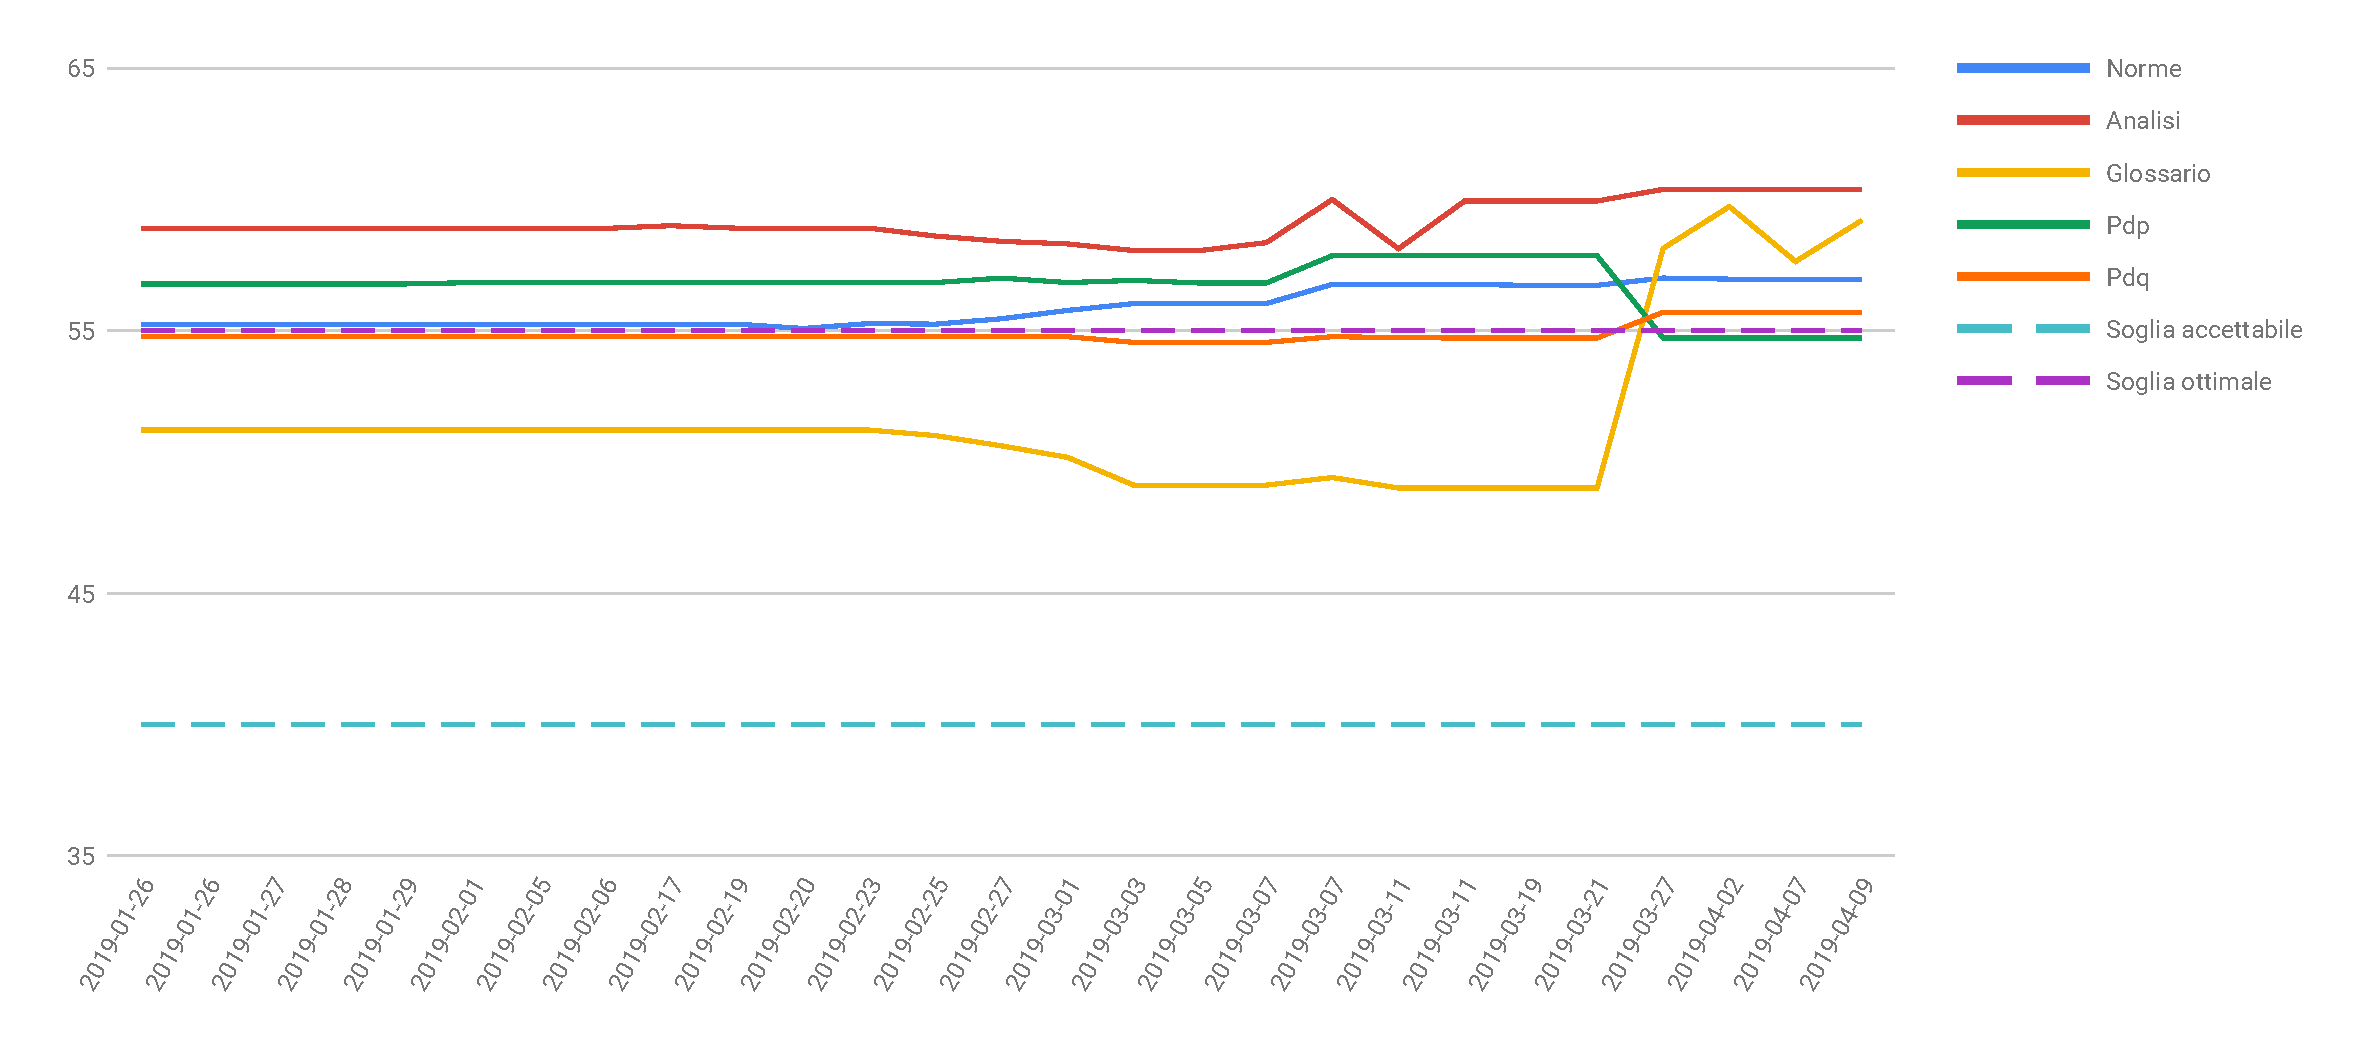
\includegraphics[width=1\linewidth]{sez/App_Esito/Qualifica/graph/gulpeaseRQ.pdf}
	\caption{Andamento dell'indice di Gulpease fino al periodo di Pianificazione e codifica}
\end{figure}
		\subsubsection{Metriche software}
			Alcune metriche per il software sono più adatte per alcuni linguaggi di programmazione e meno per altri. Come indicato nel \PdP , il gruppo \gruppo \space sceglierà quali linguaggi usare nel periodo di Progettazione Architetturale; pertanto, le metriche presenti in questa sezione non sono da considerarsi complete o definitive.\newline
Per alcune metriche, può mancare un'indicazione di valori accettabili e ottimali: ciò significa che il team si riserva di definirli in futuri incrementi.

\paragraph{Numero di Metodi}\mbox{}\\[0,3cm]
Numero medio di metodi contenuti nelle classi di un package. Un numero di metodi troppo alto può indicare la necessità di scomporre una classe. Un numero di metodi troppo basso, d'altro canto, deve far riflettere sull'effettiva utilità della classe presa in esame.\\[0,2cm]
\textbf{Parametri adottati:}
\begin{itemize}
	\item Range accettabile: $[3,9]$;
	\item Range ottimale: $[3,7]$.
\end{itemize}

\paragraph{Numero di Parametri}\mbox{}\\[0,3cm]
Numero di parametri passati a un metodo. Un eccessivo numero di parametri passati ad un metodo può indicare un'eccessiva complessità dello stesso, che va scomposto o quanto meno ripensato.\\[0,2cm]
\textbf{Parametri adottati:}
\begin{itemize}
	\item Range accettabile: $[0,8]$;
	\item Range ottimale: $[0,5]$.
\end{itemize}

\paragraph{Funzioni di interfaccia per package}\mbox{}\\[0,3cm]
Numero di funzione che un package espone. Un valore troppo elevato potrebbe indicare un errore di progettazione\\[0,2cm]
\textbf{Parametri adottati:}
\begin{itemize}
	\item Range accettabile: $[0,20]$;
	\item Range ottimale: $[0,10]$.
\end{itemize}

\paragraph{Complessità Ciclomatica}\mbox{}\\[0,3cm]
La Complessità Ciclomatica (CC) è una metrica software che misura la complessità di un programma contando il numero di cammini linearmente indipendenti attraverso il grafo di controllo di flusso. In questo grafo, i nodi corrispondono a gruppi indivisibili di istruzioni, mentre gli archi connettono due nodi se il secondo gruppo di istruzioni può essere eseguito immediatamente dopo il primo gruppo: sono quindi responsabili dell'aumento della CC i punti decisionali, \emph{if} e \emph{for}.
Tenere bassa la CC può portare a vari vantaggi:
\begin{itemize}
	\item Minore complessità durante lo sviluppo;
	\item Maggior facilità nell'aumentare la code coverage in fase di test;
	\item Maggior coesione del codice;
\end{itemize}
\textbf{Parametri adottati:}
\begin{itemize}
	\item Range accettabile: $[0,17]$;
	\item Range ottimale: $[0,10]$.
\end{itemize}

\paragraph{Campi dati per classe}\mbox{}\\[0,3cm]
Numero di campi dati contenuti da una classe. Una classe con troppi campi dati può essere sintomo di cattiva progettazione e va ripensata.\\[0,2cm]
\textbf{Parametri adottati:}
\begin{itemize}
	\item Range accettabile: $[0,15]$;
	\item Range ottimale: $[0,10]$.
\end{itemize}

\paragraph{Commenti per linee di codice}\mbox{}\\[0,3cm]
Rapporto fra le righe di codice (righe vuote escluse) e le righe di commento. Un codice ben commentato può essere compreso più facilmente e velocemente, facilitando le operazioni di manutenzione.\\[0,2cm]
\textbf{Parametri adottati:}
\begin{itemize}
	\item Range accettabile: $[10\%,100\%]$;
	\item Range ottimale: $[15\%,100\%]$.
\end{itemize}

\paragraph{Code Coverage}\mbox{}\\[0,3cm]
Percentuale delle linee di codice coperte dai test.\\[0,2cm]
\textbf{Parametri adottati:\newline}
Il gruppo \gruppo \space si riserva di decidere in futuro i parametri da adottare.

\paragraph{Superamento test}\mbox{}\\[0,3cm]
Percentuale di test superati. Per avere un prodotto di qualità, è necessario che esso superi i test prestabiliti.\\[0,2cm]
\textbf{Parametri adottati:}
\begin{itemize}
	\item Range accettabile: $[70\%,100\%]$;
	\item Range ottimale: $[95\%,100\%]$.
\end{itemize}

\paragraph{Requisiti obbligatori soddisfatti}\mbox{}\\[0,3cm]
Percentuale di requisiti obbligatori stabiliti dalla proponente soddisfatti. \'E fondamentale, per la buona riuscita del progetto, soddisfare i requisiti obbligatori individuati nell'\AdR .\\[0,2cm]
\textbf{Parametri adottati:}
\begin{itemize}
	\item Range accettabile: $[70\%,100\%]$;
	\item Range ottimale: $[95\%,100\%]$.
\end{itemize}
	

		\subsubsection{Riassunto metriche}
			%\begin{table}[H]
	\rowcolors{2}{greyROwSWEight}{white}
	\renewcommand{\arraystretch}{1.5}
	%\centering
	\begin{longtable}{C{4cm} c c c}
	
	\rowcolor{greySWEight}
	\textcolor{white}{\textbf{Codice}} &
	\textcolor{white}{\textbf{Nome}} &
	\textcolor{white}{\textbf{Accettabile}} &
	\textcolor{white}{\textbf{Ottimale}}\\
	\endhead

	%%% ENTRY
	\textbf{MD001} &
	Indice Gulpease &
	$[40 , 100] $&
	$[55 , 100]$\\

	%%% ENTRY
	\textbf{MP001} &
	Schedule Variance &
	$(-\infty , 3] $&
	$(-\infty , 0]$\\
	
	%%% ENTRY
	\textbf{MP002} &
	Budget Variance &
	$(-\infty , 9\%] $&
	$(-\infty , 1\%]$\\


	%%% ENTRY
	\textbf{MS001} &
	Numero di metodi &
	$[3 , 9] $&
	$[3 , 7]$\\
	
	%%% ENTRY
	\textbf{MS002} &
	Numero di parametri &
	$[0 , 8] $&
	$[0 , 5]$\\
	
	%%% ENTRY
	\textbf{MS003} &
	Funzioni di interfaccia per package &
	$[0 , 20] $&
	$[0 , 10]$\\
	
	%%% ENTRY
	\textbf{MS004} &
	Complessità ciclomatica &
	$[0 , 17] $&
	$[0 , 10]$\\
	
	%%% ENTRY
	\textbf{MS005} &
	Campi dati per classe &
	$[0 , 15] $&
	$[0 , 10]$\\
	
	%%% ENTRY
	\textbf{MS006} &
	Commenti per linee di codice &
	$[10\%, 100\%] $&
	$[15\% , 100\%]$\\
	
	%%% ENTRY
	\textbf{MS007} &
	Code coverage &
	$[80\%, 100\%]$&
	$[90\%, 100\%]$\\

	
	%%% ENTRY
	\textbf{MS008} &
	Superamento test &
	$[100\%, 100\%]$&
	$[100\%, 100\%]$\\
	
	%%% ENTRY
	\textbf{MS009} &
	Soddisfacimento requisiti obbligatori &
	$[100\%, 100\%]$&
	$[100\%, 100\%]$\\
	
	%%% ENTRY	
	\textbf{MS010} &
	Media di build Travis settimanali &
	$[15,\infty]$&
	$[25,\infty]$\\
	
	%%% ENTRY
	\textbf{MS011} &
	Percentuale build Travis superate &
	$[75\%,100\%]$&
	$[85\%,100\%]$\\
	
	\rowcolor{white}
	\caption{Riassunto delle metriche}\\	
	\end{longtable}


\appendix
\addcontentsline{toc}{part}{Appendici}

\newpage
\section{Esito Verifica}
	\label{app:misure}
	\subsection{Periodo di Analisi}
	\subsection{Document goal}
The purpose of this document is to provide all the necessary information to extend, correct and improve Colletta.
There will be additional information regarding setting up the development environment to work in an environment that is as consistent as possible with that used
by the other members of group SWEight, but can be ignored if you only want to use part of the product.
This guide was written taking into account the Microsoft Windows and Linux operating systems. If other systems are used, compatibility issues may arise, even if it's unlikely. In this case refer to the git page. This document will grow as the product will be fully
developed.

\subsection{Product goal}
The purpose of the product is the creation of a collaborative data collection platform where users can prepare and/or perform small grammar exercises. 
The front-end of the system consists of a web application developed with React and Redux, while the back-end is a Spring Boot application written in Java, which will handle HTTP Requests sent from the front-end. 

\subsection{References}


\subsubsection{Installation references}

\begin{itemize}
\item \textbf{Git}: \url{https://git-scm.com/}
\item \textbf{Node.js}: \url{https://nodejs.org/en/}
\item \textbf{NPM}: \url{https://www.npmjs.com/}
\item \textbf{Oracle JDK}: \url{https://www.oracle.com/technetwork/java/javase/downloads/index.html}
\item \textbf{OpenJDK}: \url{https://openjdk.java.net/}
\item \textbf{Maven}: \url{https://maven.apache.org/}
\item \textbf{Lombok}: \url{https://projectlombok.org/}
\item \textbf{VSCode}: \url{https://code.visualstudio.com/} 

\end{itemize}

\subsubsection{Legal references}
\begin{itemize}
\item \textbf{MIT License}: \url{https://opensource.org/licenses/MIT}
\end{itemize}

%\subsubsection{Informative references}

		\subsubsection{Misurazioni Documenti}
			% DA INCREMENTARE PER 
\paragraph{MD001 - Indice di Gulpease}\mbox{}\\[0,3cm]
\begin{table}[H]
	\centering
	\begin{tabular}{cccc}
	\rowcolor{greySWEight}
	\textcolor{white}{\textbf{Documento}} & 
	\textcolor{white}{\textbf{Abbreviazione}} &
	\textcolor{white}{\textbf{Valore Indice}}&
	\textcolor{white}{\textbf{Riscontro}}\\
	
	\textbf{Analisi dei Requisiti} & ADR & 60.38 & \textcolor{ForestGreen}{Ottimale} \\
	\textbf{Glossario} & GLO & 59.20 & \textcolor{ForestGreen}{Ottimale} \\
	\textbf{Piano di Qualifica} & PDQ & 55.70 & \textcolor{ForestGreen}{Ottimale} \\
	\textbf{Piano di Progetto} & PDP & 54,72 & \textcolor{YellowOrange}{Accettabile} \\
	\textbf{Norme di Progetto} & NDP & 56,96 & \textcolor{ForestGreen}{Ottimale} \\

	\end{tabular}
	\caption{Indice di Gulpease nel periodo di codifica}
\end{table}

\begin{figure}[H]
	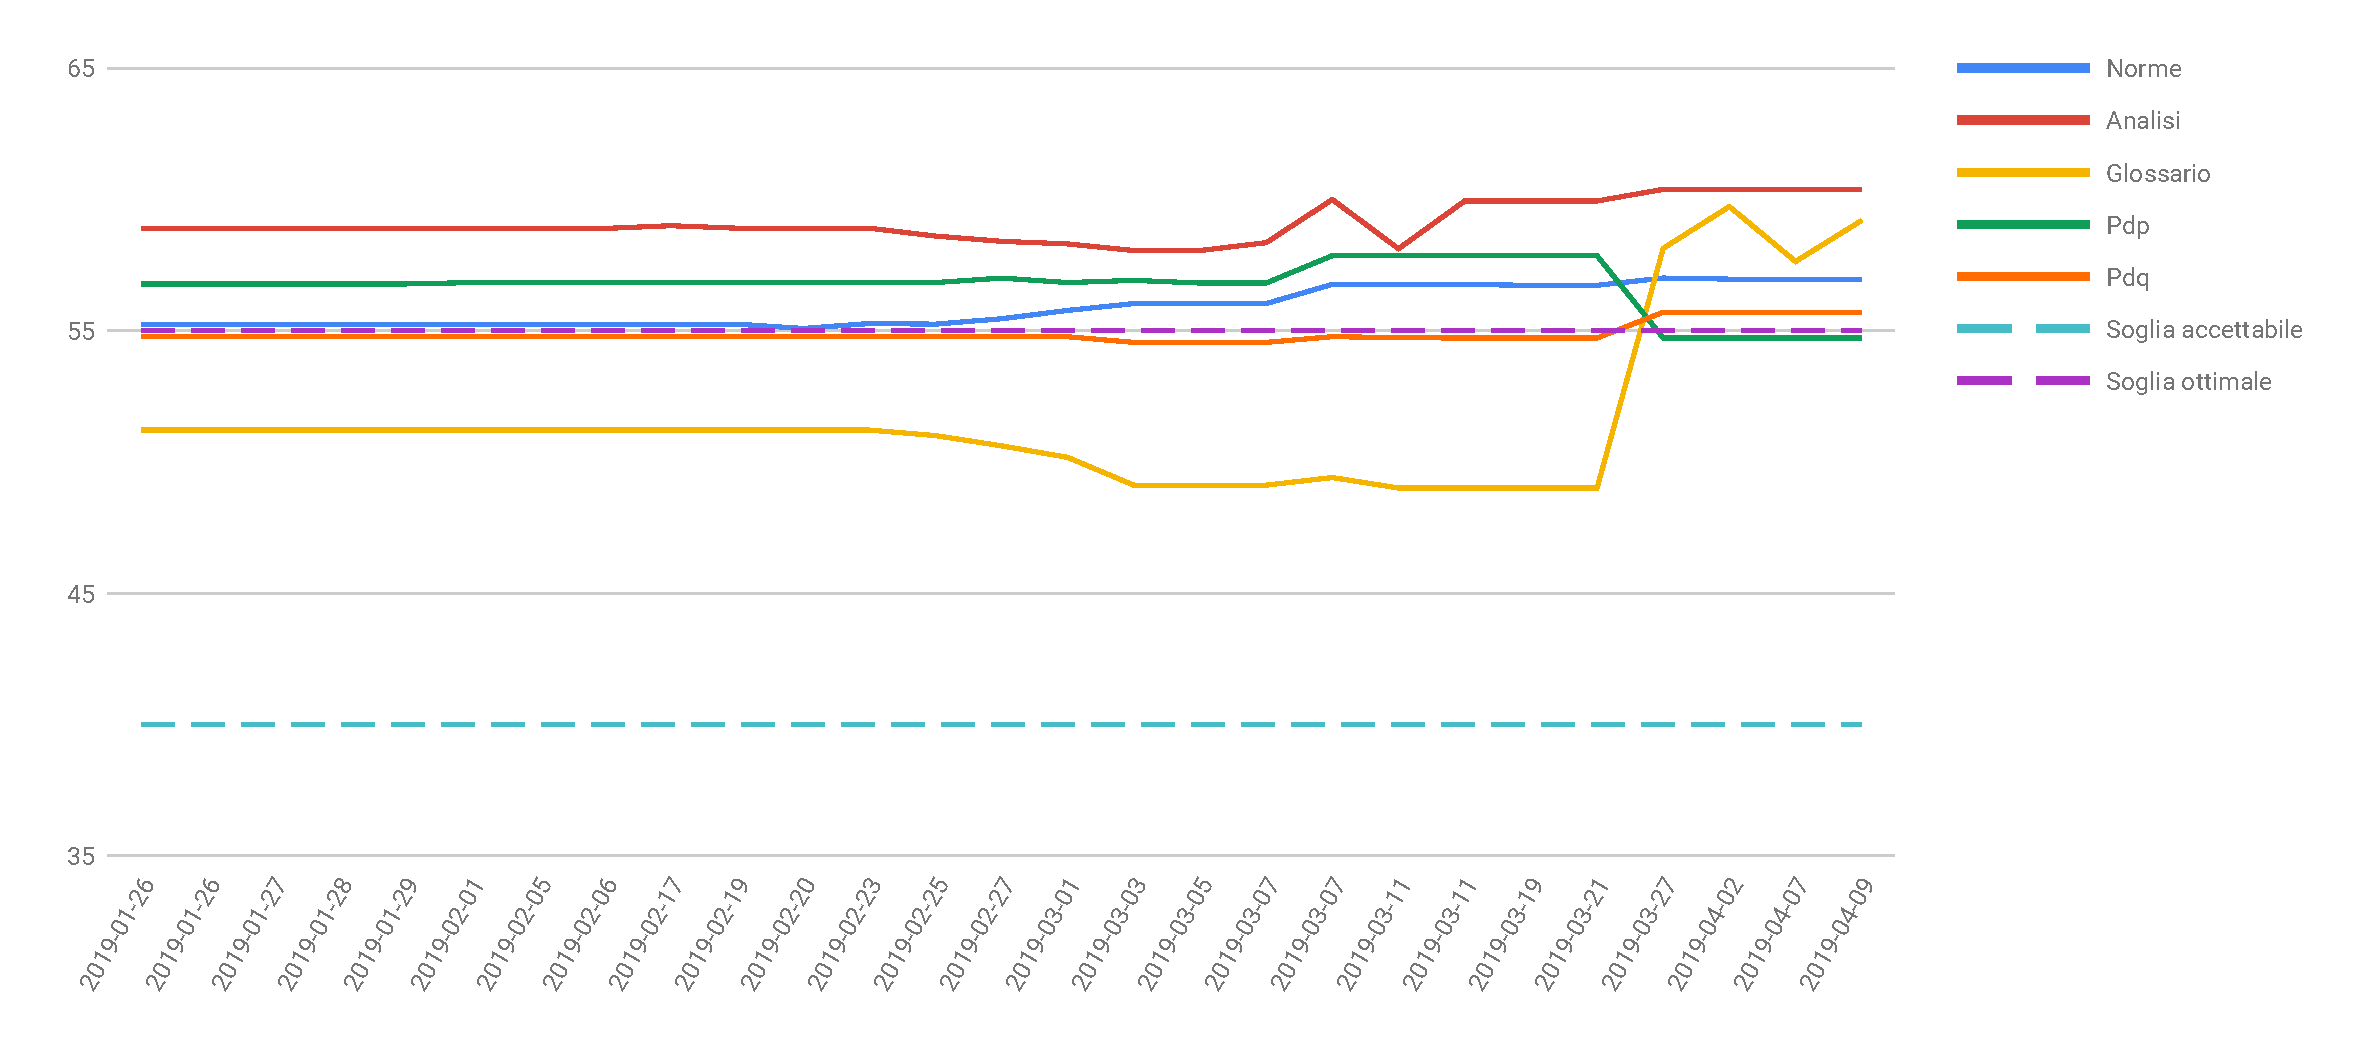
\includegraphics[width=1\linewidth]{sez/App_Esito/Qualifica/graph/gulpeaseRQ.pdf}
	\caption{Andamento dell'indice di Gulpease fino al periodo di Pianificazione e codifica}
\end{figure}
		\subsubsection{Misurazione Processi}
			Le metriche presentate in questa sezione monitorano lo stato dei processi del progetto analizzando l'uso che essi fanno di tempo e risorse finanziarie. Sono particolarmente utili per il \Res , che può quindi decidere di apportare modifiche alla pianificazione quando necessario.

\paragraph{MP001 - Schedule Variance}\mbox{}\\[0,3cm]
La Schedule Variance indica se una certa attività o processo è in anticipo, in pari, o in ritardo rispetto alla data di scadenza prevista\\[0,2cm]
\textbf{Parametri adottati:}
\begin{itemize}
	\item Range accettabile: $(-\infty , 3]$;
	\item Range ottimale: $(-\infty , 0]$.
\end{itemize}

\paragraph{MP002 - Budget Variance}\mbox{}\\[0,3cm]
La Budget Variance misura, ad una determinata data, lo scostamento fra quanto speso e quanto preventivato. \\[0,2cm]
\textbf{Parametri adottati:}
\begin{itemize}
	\item Range accettabile: $(-\infty , 9\%]$;
	\item Range ottimale: $(-\infty , 1\%]$.
\end{itemize}
		\subsubsection{Retrospettiva}
			
Riepilogo delle attività che necessitano di ulteriori spiegazioni:
\begin{itemize}
    \item \textbf{Scedule Variance}: Le attività hanno subito dei brevi ritardi che sono da cosiderarsi accettabili;
    \item \textbf{Metriche software}: Per ogni tabella delle metriche software in appendice, è stato inserito 
    il numero di file sui quali essa è stata valutata.
    Questo perchè per evidenti motivi non tutte le metriche erano adatte ad essere utilizzate anche 
    sui file di frontend;
    \item \textbf{Requisiti obbligatori}: Molti dei requisiti obbligatori che abbiamo segnato come non 
    soddisfatti in realtà sono stati parzialmente realizzati, infatti sono già stati implementati nel
    backend ma non ancora nel frontend. Riteniamo inoppugnabile la certezza che verranno tutti portati 
    a termine nella Revisione di Approvazione;
    \item \textbf{Travis}: Il valore minimo accettabile prefissato per le build superate era del 75\%, il valore riscontrato
    è 71.40\%, questo potrebbe implicare la presenza di errori. Dato che le percentuali delle
    build superate delle ultime due settimane corrisponde al 85.15\%, il valore finale
    trovato non rispetta i valori prestabiliti a causa della poca esperienza di codifica di inizio periodo.
\end{itemize}

\newpage
\section{Pianificazione Test}
	\subsection{Document goal}
The purpose of this document is to provide all the necessary information to extend, correct and improve Colletta.
There will be additional information regarding setting up the development environment to work in an environment that is as consistent as possible with that used
by the other members of group SWEight, but can be ignored if you only want to use part of the product.
This guide was written taking into account the Microsoft Windows and Linux operating systems. If other systems are used, compatibility issues may arise, even if it's unlikely. In this case refer to the git page. This document will grow as the product will be fully
developed.

\subsection{Product goal}
The purpose of the product is the creation of a collaborative data collection platform where users can prepare and/or perform small grammar exercises. 
The front-end of the system consists of a web application developed with React and Redux, while the back-end is a Spring Boot application written in Java, which will handle HTTP Requests sent from the front-end. 

\subsection{References}


\subsubsection{Installation references}

\begin{itemize}
\item \textbf{Git}: \url{https://git-scm.com/}
\item \textbf{Node.js}: \url{https://nodejs.org/en/}
\item \textbf{NPM}: \url{https://www.npmjs.com/}
\item \textbf{Oracle JDK}: \url{https://www.oracle.com/technetwork/java/javase/downloads/index.html}
\item \textbf{OpenJDK}: \url{https://openjdk.java.net/}
\item \textbf{Maven}: \url{https://maven.apache.org/}
\item \textbf{Lombok}: \url{https://projectlombok.org/}
\item \textbf{VSCode}: \url{https://code.visualstudio.com/} 

\end{itemize}

\subsubsection{Legal references}
\begin{itemize}
\item \textbf{MIT License}: \url{https://opensource.org/licenses/MIT}
\end{itemize}

%\subsubsection{Informative references}

	
\newpage
\section{Qualità}
	\subsection{SPICE}
		\label{app:SPICE}
		Il modello ISO/IEC 1554, meglio conosciuto come SPICE (Software Process Improvement and Capability Determination), è lo standard di riferimento per valutare in modo oggettivo la qualità dei processi nello sviluppo del software. \newline
Sono definiti:
\begin{itemize}
	\item Una serie di \textbf{attributi} per ogni processo, che ne vanno a determinare la sua capability (capacità):
	\begin{itemize}
	    \item Process performance;
	    \item Performance management;
	    \item Work product management;
	    \item Process definition;
	    \item Process deployment;
	    \item Process measurement;
	    \item Process control;
	    \item Process innovation;
	    \item Process optimization;
	\end{itemize}
	
	Ognuno di questi attributi riceve una valutazione nella seguente scala:
	\begin{itemize}
	    \item \textbf{N: }Non raggiunto (0 - 15\%);
	    \item \textbf{P: }Parzialmente raggiunto (>15\% - 50\%);
	    \item \textbf{L: }Largamente raggiunto (>50\%- 85\%);
	    \item \textbf{F: }Pienamente raggiunto (>85\% - 100\%);
	\end{itemize}
	\item Sei \textbf{livelli di capacità} dei processi:
		\begin{enumerate}[start=0]
			\item Incompleto;
			\item Eseguito;
			\item Gestito;
			\item Stabilito;
			\item Predicibile;
			\item Ottimizzato;
		\end{enumerate}
	\item Delle linee guida per effettuare delle \textbf{stime}, eseguite tramite:
		\begin{itemize}
			\item \textbf{Processi di misurazione}, descritti nel \PdP ;
			\item \textbf{Modello di misurazione}, descritto in questo documento;
			\item \textbf{Strumenti di misurazione}, descritti nelle \NdP ;
		\end{itemize}
	\item Una serie di \textbf{competenze} che chi effettua misurazioni deve possedere. La mancanza di esperienza degli elementi del gruppo \gruppo , fa sì che nessun membro possieda queste skill, rendendo così impossibile la piena adesione allo standard. Tuttavia, ogni componente è chiamato a studiare SPICE e a applicare al meglio le indicazioni descritte in questo documento e nelle \NdP , al fine di perseguire un livello di qualità accettabile.
	
\end{itemize}

	\subsection{ISO/IEC 9126}
		\label{app:ISO/IEC 9126}
		Lo standard ISO/IEC 9126 stabilisce una serie di linee guida mirate al miglioramento delle qualità del software sviluppato.

\begin{figure}[H]
  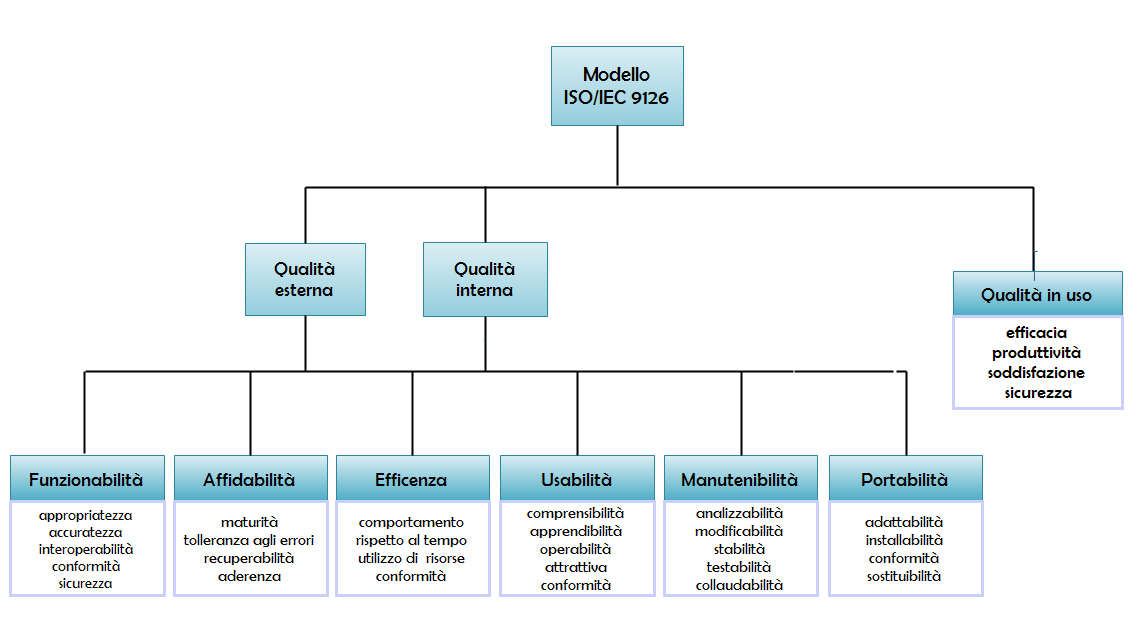
\includegraphics[width=\linewidth]{sez/App_Qualita/grafico_9126.png}
  \caption{Rappresentazione grafica di ISO/IEC 9126 [Wikipedia]}
  \label{fig:9126}
\end{figure}

Come presentato in \autoref{fig:9126}, ISO/IEC 9126 prescrive indicazioni su:
\begin{itemize}
	\item \textbf{Qualità interna: }è misurata sul software non eseguibile, come, ad esempio il codice sorgente. Le misure effettuate permettono di avere una buona previsione della qualità esterna.
	\item \textbf{Qualità esterna: }è misurata tramite l'analisi dinamica su software eseguibile. Le misure effettuate permettono di avere una buona previsione della qualità in uso prodotto.
	\item \textbf{Qualità in uso: }definita in base all'esperienza utente. Sono da perseguire i seguenti obiettivi:
		\begin{itemize}
			\item Efficacia;
			\item Produttività;
			\item Soddisfazione;
			\item Sicurezza.
		\end{itemize}
\end{itemize}

ISO/IEC 9126 definisce inoltre una serie di requisiti da soddisfare per produrre software di qualità:
\begin{itemize}
	\item \textbf{Funzionalità: }capacità di un prodotto software di soddisfare le esigenze stabilite (vedi \AdR);
	\item \textbf{Affidabilità: }capacità di un prodotto di mantenere un determinato livello di prestazioni in date condizioni d'uso per un certo periodo;
	\item \textbf{Efficienza: }capacità di un prodotto software di eseguire il proprio compito minimizzando il numero di risorse usate;
	\item \textbf{Usabilità: }capacità del prodotto software di essere utilizzato, capito e studiato dall'utente a cui è rivolto;
	\item \textbf{Manutenibilità: }capacità del prodotto software di evolvere mediante modifiche, correzioni e miglioramenti;
	\item \textbf{Portabilità: }capacità del prodotto software di funzionare ed essere installato su più ambienti hardware e software.
\end{itemize}

\end{document}
